\chapter{Physical System}
\label{sec:PhysicalSystem}
We consider a two-dimensional SNS-junction in the $xy$-plane and parallel to the $x$-axis, with the interfaces placed at $x=-L/2$ and $x=L/2$. The width of the junction is $W$, see figure \ref{fig:Explaination}. The quasiparticle waves are represented by the four-component vectors $\Psi(x,y) = \big(\vec{u}(x,y) \ \ \vec{v}(x,y) \big)^T$ as used in the Bogoliubov equations \eqref{BdG-2}. We consider s-wave superconductors such that the gap parameter, $\Delta(x)$, is position-independent in each superconductor. The left and right superconductors are assumed to be of the same material, so that the magnitude, $\Delta_0$, of the gap parameter is the same in both superconductors. However, we allow the gap parameter to have different phases, $\phi_L$ and $\phi_R$, in the left and right superconductor, respectively. Necessarily, the gap parameter is zero in the normal metal. The overall gap parameter is
\begin{equation}
    \Delta(x) = \Delta_0\left( e^{i\phi_L}\Theta(-L/2-x) + e^{i\phi_R}\Theta(x-L/2)\right),
\end{equation}
where $\Theta(x)$ is the Heaviside step function. 
The Hamiltonian will be on the form given in equation \eqref{Ham-2-4}. We allow for different chemical potential, $\mu_S$ and $\mu_N$, but we assume the effective mass to be equal in the superconductor and the normal metal, i.e. $m_S = m_N \equiv m$. Moreover, we let $V(x)$ be a delta-potential barrier at the interfaces and allow for different strength, i.e. $V(x) = V_L\delta(x+L/2) + V_R\delta(x-L/2)$. The overall Hamiltonian is
\begin{equation}
    h(x,y) = h_S(x,y)\big(\Theta(-L/2-x) + \Theta(x-L/2) \big) + h_N(x,y)\Theta(x+L/2)\Theta(L/2-x) + V_L\delta(x) + V_R\delta(x-L)
\label{Ham-3}
\end{equation}
where the Hamiltonian in the superconductors (S) and normal metal (N) is given as
\begin{equation}
    h_{S/N}(x,y) = \frac{1}{2m}\left(-i\hbar\nabla-q\fet{A}(x,y)\right)^2-\mu_{S/N}
\end{equation} 
and $\fet{A}$ is the vector potential allowing for an external magnetic field.
\\
\\
We will consider the semiclassical limit $k_FL \gg 1$, in which the Andreev bound states can be associated with classical trajectories, as illustrated in figure \ref{fig:Explaination}. These trajectories can be thought of as single-mode waveguides connecting the two superconductors !!!REF!!!. We will focus the circular Fermi surface with isotropic dependence on the wave vector $\fet{k} = (k_x,k_y) = (k_F\cos\theta_k,k_F\sin\theta_k)$. We will work in the short-junction regime $L<<\xi$, with $\xi=\hbar v_f/\Delta$ the superconducting coherence length induced by the proximity effect !!!CITE!!!.
\\
\\
In the preceding chapters we will look at three different situations. First, in section \ref{sec:without} and \ref{sec:CurrentWithout}, we will consider the system without external field or barriers at the interfaces. Next, in section \ref{sec:withBarriers} and \ref{sec:CurrentWithBarriers}, we will include the barriers at each interface, but keep the external field off. Finally, in section \ref{sec:withB} and \ref{sec:CurrentWithB}, we will include an external field, but have transparent barriers. The situations without the external field is well known !!!REF!!! and will be used for comparison. There has also been research on the situation with a uniform external magnetic field, both for one-dimensional and two-dimensional systems !!!REF!!!. However, we will also consider modulated magnetic fields, which has not yet been explored. Our strategy in all three situations is to first find the ABS-energies (chapter \ref{sec:energies}) and use this result to find the Josephson current (chapter \ref{sec:current}).

\begin{figure}[hhh]
\centering
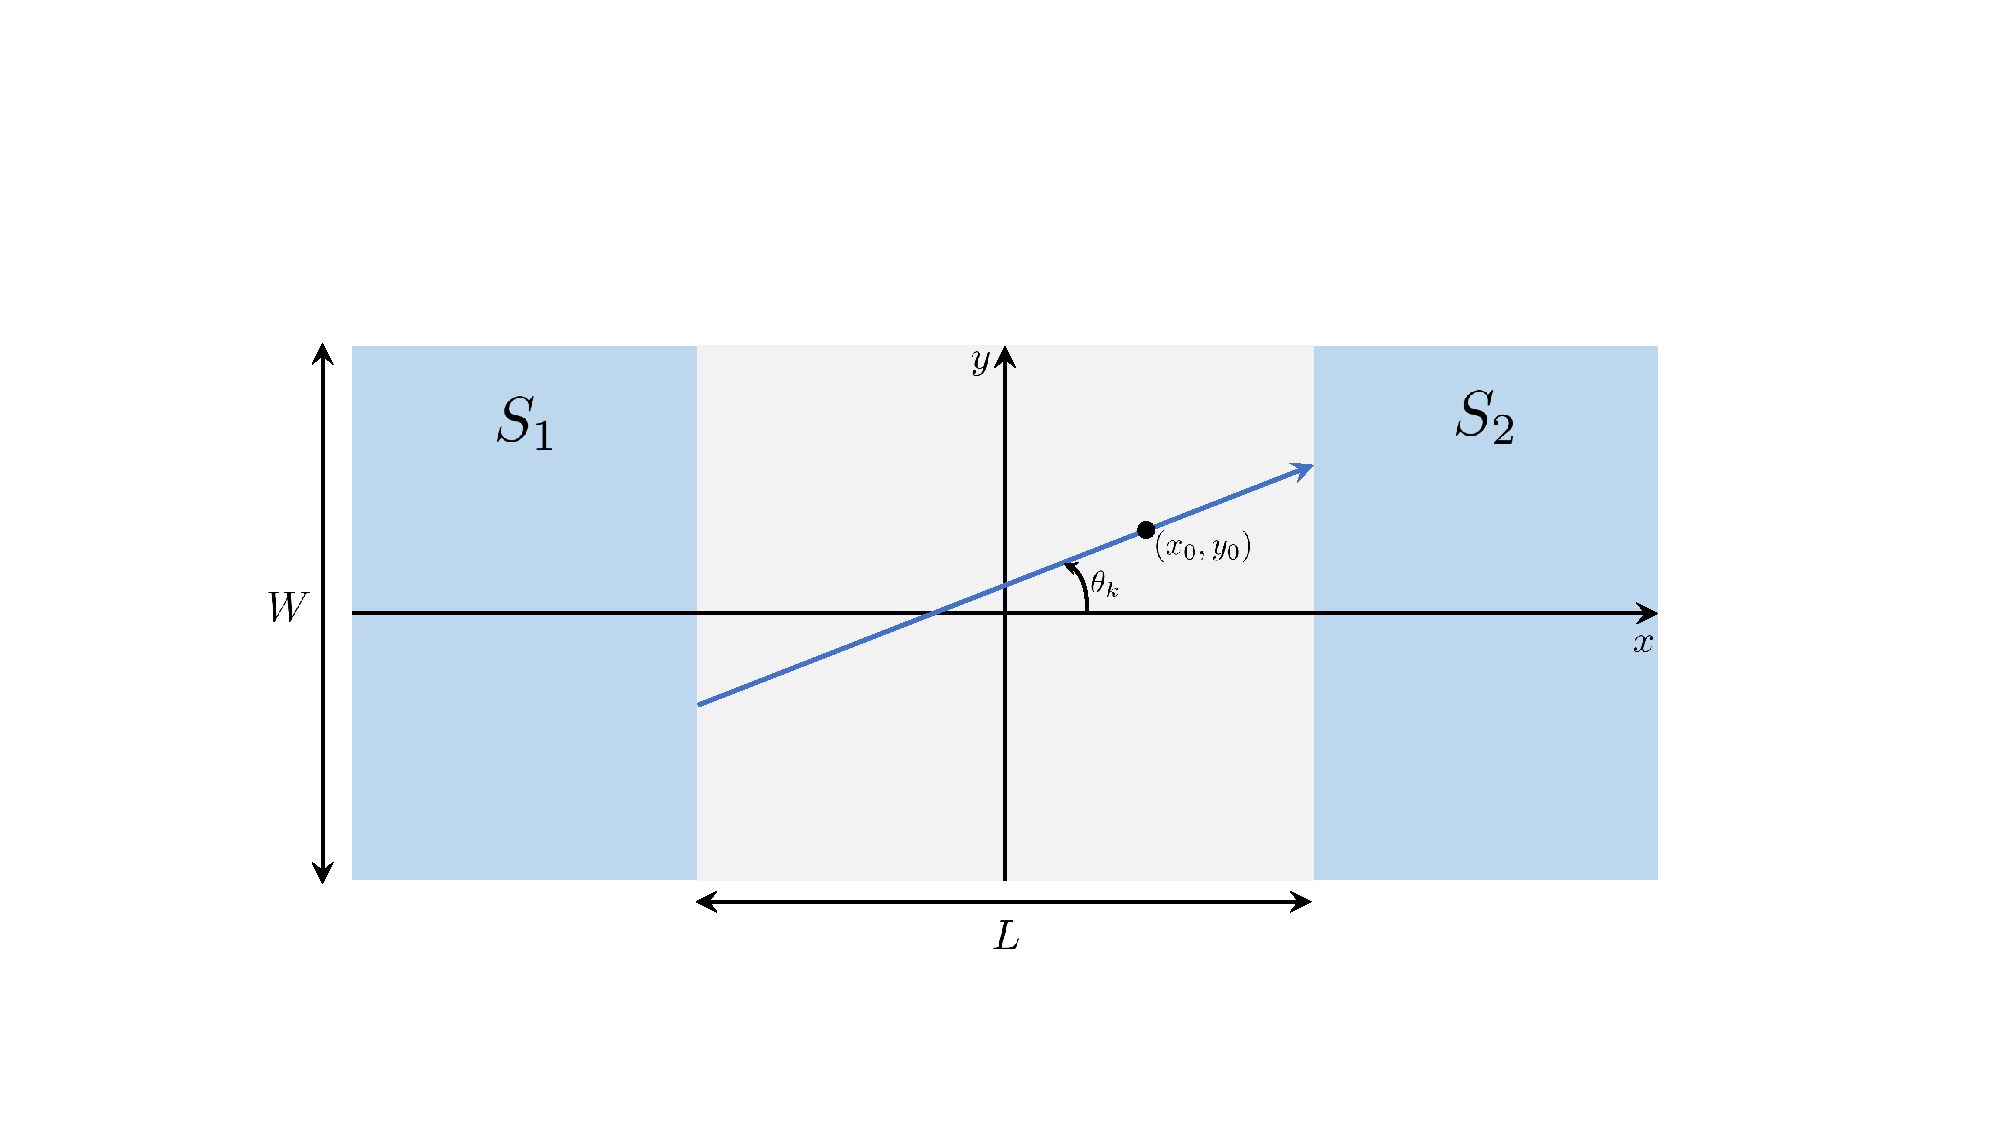
\includegraphics[width=15cm,trim = 4cm 3cm 5cm 5.5cm, clip=true ]{fig/Explaination}
\caption{blabla}
\label{fig:Explaination}
\end{figure}